\documentclass{article}
\usepackage[a4paper, margin=2.5cm]{geometry}
\usepackage[T1]{fontenc}
\usepackage[utf8]{inputenc}
\usepackage{graphicx}
\usepackage{url}
\usepackage{listings}
\usepackage{parcolumns}
\graphicspath{ {./images/} }
 
\title{Spectre \& Meltdown \\
\large{Speculative execution - performance hack or a massive vulnerability? \\ CS4028 Security: In-course assessment}}
\author{Konrad Dryja \\ 51552177 \\ k.dryja.15@abdn.ac.uk \\ University of Aberdeen}
\date{\today}
 
\begin{document}
 
\maketitle
 
\tableofcontents

\begin{abstract}
  As part of my CS4028 assessment, I would like to delve into the Spectre \& Meltdown vulnerabilities. I recognize that those are not offensive technology or tool per se, although they both expose a major flaw which could easily be applied in one of them. I found researching this subject very interesting, as it taught me a lot about low-level CPU operations and how speculative execution can be used in nefarious ways. 
\end{abstract}
 
\section{Introduction}
 
The computing and security environments were shook in January 2018 when Google's Project Zero collaborating with security researchers discovered a major flaw in almost all consumer CPUs. The vulnerabilities allowed potentially a piece of code with no special privileges to read memory outside its own sandboxed environment (or even reading privileged parts of kernel memory). Day-to-day users perhaps wouldn't be impacted to a tremendous extent, but imagine running a production server in GCP, AWS or other major cloud provider - and having other malicious actors being able to access your data from their own, virtualised containers - that's how serious the discovery was. 

\begin{figure}[h]
\centering
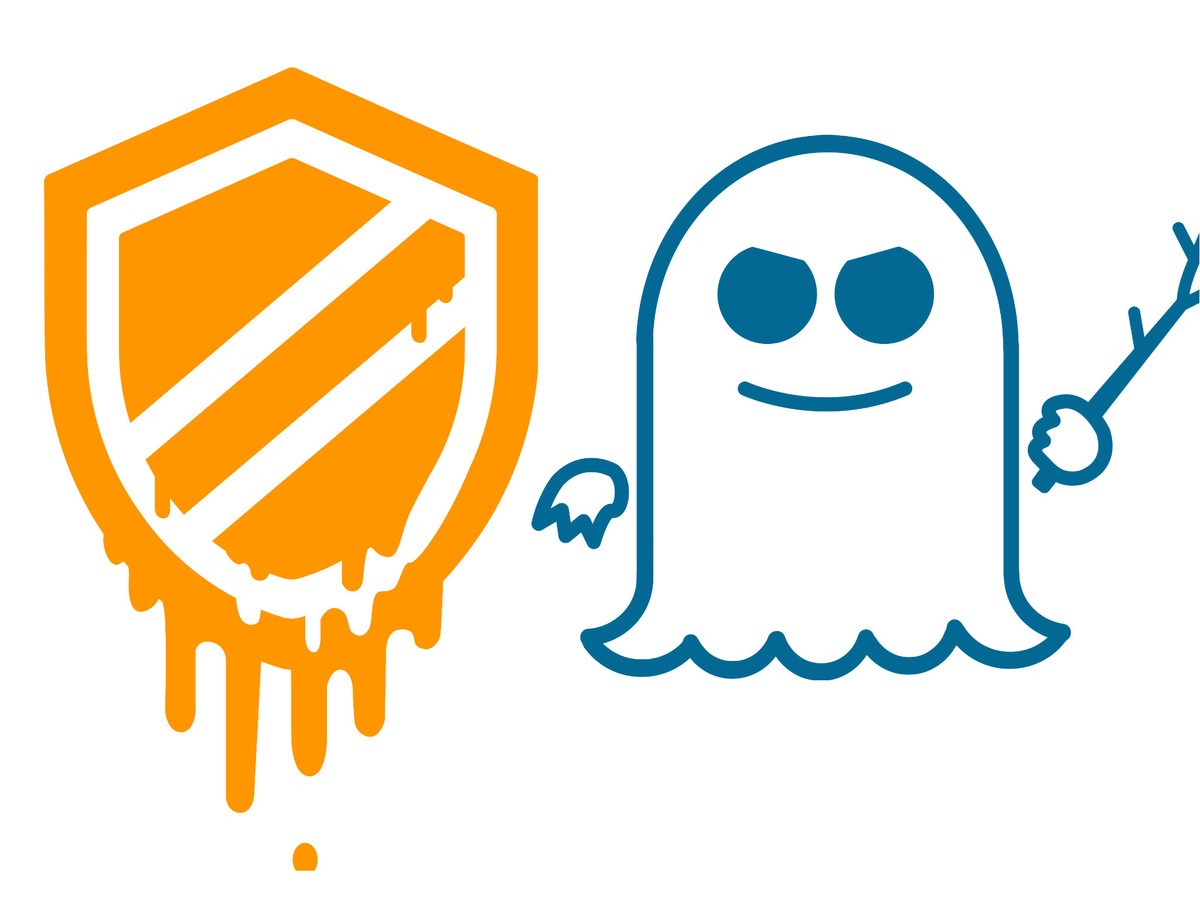
\includegraphics[width=0.3\textwidth]{logo}
  \caption{Graphic for Meltdown on the left, Spectre on the right.}
\end{figure}

The first discovery consisted of Spectre variant 1 \& 2, which was allocated Common Vulnerabilities and Exposures ID codes of CVE-2017-5753 and CVE-2017-5715 along with variant 3, which was dubbed Meltdown, with code CVE-2017-5754.
 
Moreover, the discovery spawned a slightly bigger family of vulnerabilities called Branch Target Injection or Side-Channel Attacks. The whole premise is using a covert channel to send the information back to the attacker. Ever since the announcement, there's been numerous variations, each of them defeating the previous software mitigations. Probably, one of the most recent examples being NetCAT - capable of spying on SSH sessions within the same network. This is caused also by the fact that lot of information is cached first on L-cache (more about it later), which later is sent back via a covert channel. 

And most terrifyingly, the vulnerability is serious and powerful enough that simply loading a malicious JS file is enough to leak kernel data back to the attacker.

\section{Background}

In order to understand how the vulnerabilities work, it is necessary to introduce some concepts and ideas that CPU manufacturers opted in for, also to overview low-level architecture of modern processors. In short, the biggest problems relate to Out of Order Execution (OOE), Branch Prediction (BP) and Branch Target Buffer (BTB) - all of those, in a way, were a mean to increase the performance of the chips and stand out on the market. At one point, Intel, AMD, ARM and more hit the ceiling with the clock speed, so they started seeking extra solutions - Branch Prediction was one of them. 

\paragraph{Branch Prediction}
To explain BP, I'm going to use an analogy one of the Stack Overflow users has introduced \cite{BranchpredictionSO}. The original poster discovered that simple array operation is significantly faster when the data is sorted, compared to unsorted - which at first seems like a compiler optimization, but eventually it was established that this artifact persists throughout different compilers, languages or environments. 

\noindent\begin{minipage}{.45\textwidth}
\begin{lstlisting}[caption=Operation on an unsorted array,frame=tlrb]{Name}
from random import randint
arr = [randint(0,100) 
  for x in range(1000)]
# Start measuring time here
for y in range(1000000):
  for x in arr:
    if x > 50:
      print("more than 50")
\end{lstlisting}
\end{minipage}\hfill
\begin{minipage}{.45\textwidth}
\begin{lstlisting}[caption=Operation on a sorted array,frame=tlrb]{Name}
from random import randint
arr = [randint(0,100) 
  for x in range(1000)]
arr = sorted(arr)
# Start measuring time here
for y in range(1000000):
  for x in arr:
    if x > 50:
      print("more than 50")
\end{lstlisting}
\end{minipage}

Consider Listing 1 \& 2. Disregarding the time needed for sorting the array, seemingly the for-loop on Listing 2 was much faster, the difference was quite major too, reaching an order of magnitude improvement of even 1s with branch prediction and 10s without. Finally, it was determined that it's not the compiler optimizing the machine code - but rather the CPU itself. Imagine the CPU being a very heavy train, which takes a lot of time to get it started and lot of time to have it stopped. Our job, as an operator at the intersection, is to determine whether to flip the lever and change the direction of the tracks. Now assume that the past 50 trains took the route to the left and we have 51st train approaching. We can make educated guess and let the train preemptively go towards the left. Best case - we save a lot of time and train keeps going in the correct direction. Worst case, the train has to stop, roll back and go towards the right. Then we reflect on it and apply the finding during the future incidents.

Machine code is split into many branches - conditions. To increase performance, CPU will ``predict`` the outcome of the next operation, such that it'd be ready inside L-cache while a heavy operation (for example IO) is still pending. But, in a situation where the prediction is incorrect, the operation is rolled back. 

\paragraph{Out of Order execution}
The technique is very similar to BP, in a way, as the ultimate goal is to speed up execution of instructions. It is a way to re-order and optimize the tasks to minimize the waiting time. I'd like to also point out the existence of \textbf{CPU cache} (also known as L-cache). Modern computers can store long-standing, persistent data on Solid State or spinning Drives, OS will often load and store running application within RAM. But access to either is going to be horribly slow, considering that modern CPUs run at clock speed of over 3GHz, which is 3000000000 clock cycles every second. To avoid the wait for data to arrive from external sources, cores often have built-in, small and incredibly fast memory called L1, L2 \& L3 cache.

Imagine a simple program consisting of the following steps:
\begin{enumerate}
  \item Load X
  \item Load Y, Z
  \item Sum X, Y, store it in K
  \item Sum Y, Z, store it in V
  \item Sum K, V
\end{enumerate}

Let's also assume that Y and Z are already present in the CPU cache, but X will need to be retrieved from RAM. For the sake of the example, the former operation takes 1 CPU cycle and the latter takes 3 (in reality though, the difference is much, much, much greater).

\begin{figure}[ht]
\centering
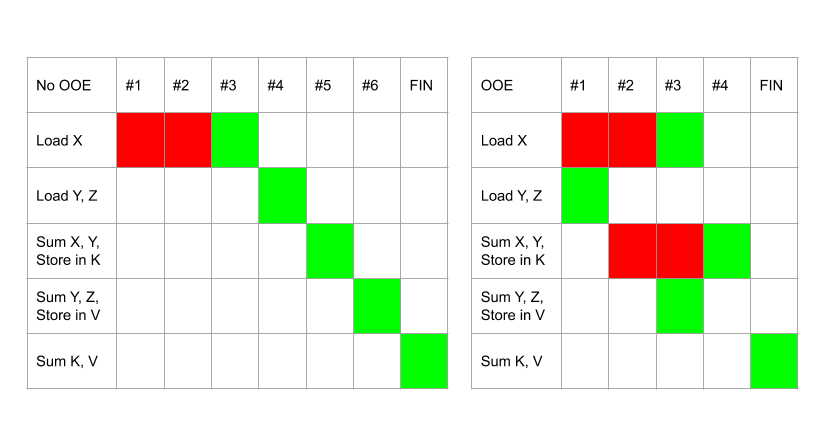
\includegraphics[width=0.9\textwidth]{OOE}
  \caption{OOE optimization}
\end{figure}

As per Figure 2, the execution would be halted at the first step, in order to retrieve the X from RAM, with the entire program taking 7 cycles. On the other hand, OOE optimizer would recognize the blocker and execute step 2 \& 4 \textbf{before} even reaching that point. That way, the entire operation can be closed only in 5 cycles, thus improving the execution speed by 25\%. As mentioned before, in reality RAM access is much slower, so that difference ends up being much more significant.

\section{Meltdown \& Spectre}
 
Having covered the background behind the attack and feature it exploits, we can finally progress to the description itself. As mentioned at the beginning of the paper, it is necessary to distinct between Meltdown and Spectre, as ultimately they reach a different goal. Together, they are part of "branch target injection" class of vulnerabilities. The most impressive and scariest part is that in no way it exploits any of the software flaws, nor it is easy or even possible to patch it. Official recommendation by CERT Coordination Center \cite{Replacement} is to completely replace the hardware with newer revisions with revised architecture no longer susceptible to those kind of attacks.

I'd like to present two different examples, as described in the original papers \cite{kocher2018spectre}\cite{lipp2018meltdown} released by Google's Project Zero. First would be a simple C program with the capability of reading privileged data, which otherwise would not be accessible and any attempts would result in either segmentation or page faults.
The other - an attack on JavaScript interpreter on a browser with site-isolation disabled (Spectre mitigation). Which in theory means, that simply loading malicious website and executing the code would be enough to leak sensitive information from the computer. 


\paragraph{Meltdown}
Let's first though clear the disambiguation between the two. As we might know, the kernel is utilizing its own page table, which should never be accessible by the user. This holds information such as passwords, keyrings or other privileged information - important for running of the system (e.g. TLS connections). This would only be available when context switch happens into the kernel mode.

To increase the performance, modern CPU manufacturers map the kernel page-table space to every running process. This speeds up context switching and limits page faults. Of course, the address space is scrambled and protected by privileged bit meaning any access attempts will result in denials - and that's where speculative execution comes in action. Combination of Branch Prediction and Out of Order Execution gives the attacker the power to retrieve arbitrary data given memory location with reasonable throughput.

% \pagebreak
\begin{lstlisting}[caption=Meltdown PoC,frame=tlrb, numbers=left, firstnumber=1]{Name}
char testArray[256 * 64];
evictCache(testArray);
char x = * kernelSpace; // Will cause segmentation fault
testArray[x * 64]++; // Will be executed speculatively
for(int i=0; i<256; i++) {
  if(is_cached(testArray[i * 64]) {
    // Cache hit! Found secret bit.
  }
}
\end{lstlisting}

In Listing 3, I have included a very high overview of the idea behind Meltdown. I will try to explain everything line-by-line before jumping into a real Proof-of-Concept working example.
\begin{enumerate}

  \item [1] Let's start with initiating our testArray - that's the entity that we're going to use to detect privileged information. We're planning to store 256 elements in it - and since L-cache is usually divided into rows 64-bits each, we multiply it by that number. 
  \item [2] We want to evict all current information residing in L-cache. This step highly depends on architecture and used compiler, usually it is achieved by writing large quantities of junk directly to the CPU.
  \item [3] Normally, we'd be looking to wrap line 3 and 4 in a try-catch block, as in 3rd line, we'd be attempting to access privileged information, causing segfault - so execution of the program would be dropped and all results discarded.
  \item [4] Assuming the information from previous step, the CPU tries to optimize the execution and \textbf{predicts} that line 5 won't segfault, thus reordering the execution flow, running the operation early and saving the results in L-cache. But, once the clock actually reaches the forbidden operation, the results are discarded and rolled back, showing the fault. Though the results are still in cache...
  \item [5-9] This is the crucial and last step in the whole operation. We're simply iterating over all elements of our testArray and measuring the access time. is\_cached()'s job would be to tell us how long it takes to retrieve given bit from the array. As retrieval from L-cache is significantly faster, we can make an assumption that the operation was indeed speculatively executed and the secret bit was leaked... Repeat for the rest of the array.

\end{enumerate}

Having explained the absolute basics behind the attack, let's try executing a real-life proof-of-concept showcasing the possibilities. I will be using code produced by Pavel Boldin\cite{MeltdownPOC}. For reference, here are the parameters of the computer that I used for the test:

\begin{quote}
\% uname -a 
\\ $>$ Linux workstation 5.3.5-arch1-1-ARCH \#1 SMP PREEMPT Mon Oct 7 19:03:08 UTC 2019 x86\_64 GNU/Linux 
\\ \% lscpu | grep name
\\ $>$ Model name: Intel(R) Core(TM) i5-6500 CPU @ 3.20GHz
\end{quote}

Additionally, since the vulnerability was already patched, I was able to disable those mitigations, as the option to do so has been available since Linux 5.2 - the choice is mostly offered due to the great performance impact of the subsequent patches \cite{low2018overview}. The PoC that I'm about to run is going to access \lstinline{linux_proc_banner} - normally located in privileged, kernel space. Note: for the purposes of the experiment, the code is run with sudo privileges to determine the exact address space, as normally KASLR (Kernel Address Space Layout Randomization) will scramble it upon every reboot - although there have already been successful attempts at breaking that security ``feature`` as well \cite{jang2016breaking} - normally, even knowing the exact memory location, access shouldn't be allowed. 


\begin{lstlisting}[caption=Meltdown in action, frame=tlrb, breaklines=true]{Name}
% sudo ./run.sh          
read ffffffffbbc00140 = 25 % (score=963/1000)
read ffffffffbbc00141 = 73 s (score=983/1000)
read ffffffffbbc00142 = 20   (score=983/1000)
read ffffffffbbc00143 = 76 v (score=993/1000)
read ffffffffbbc00144 = 65 e (score=60/1000)
read ffffffffbbc00145 = 72 r (score=997/1000)
read ffffffffbbc00146 = 73 s (score=986/1000)
read ffffffffbbc00147 = 69 i (score=971/1000)
read ffffffffbbc00148 = 6f o (score=648/1000)
read ffffffffbbc00149 = 6e n (score=42/1000)
read ffffffffbbc0014a = 20   (score=992/1000)
read ffffffffbbc0014b = 25 % (score=969/1000)
read ffffffffbbc0014c = 73 s (score=995/1000)
read ffffffffbbc0014d = 20   (score=986/1000)
read ffffffffbbc0014e = 28 ( (score=991/1000)
read ffffffffbbc0014f = 62 b (score=977/1000)
\end{lstlisting}


\begin{lstlisting}[caption=init/version.c from Linux kernel source code, frame=tlrb, breaklines=true]{Name}
const char linux_proc_banner[] =
	"%s version %s"
	" (" LINUX_COMPILE_BY "@" LINUX_COMPILE_HOST ")"
	" (" LINUX_COMPILER ") %s\n";
\end{lstlisting}

Upon completion, a dump of the banner is displayed in stdout. For comparison, Listing 5 includes snippet from Linux's source code \cite{linuxsrc} showing the exact value and location of the banner. 

\paragraph{Spectre}
Variant 1 \& 2 are abusing the same optimizers as Meltdown (Variant 3), that is, similar technique is used - measuring how quick the read times are to calculate whether we're hitting CPU cache or not. The two and the most significant differences would be:

\begin{itemize}
  \item As opposed to Meltdown, Spectre is capable of crossing the process boundaries and access memory of other software currently running on the system. Think, for example, malicious software running inside a Virtual Machine capable of accessing memory in the host OS. Or to refer to the previous situation with cloud providers - potentially attacker could access other VMs running on the same cluster / machine.
  \item And finally, whereas Meltdown was found out to be susceptible only on Intel's architecture, Spectre has been successfully reproduced in all major architectures from AMD, Intel, ARM and more. 
\end{itemize}

\begin{lstlisting}[caption=Spectre PoC,frame=tlrb, numbers=left, firstnumber=1, float]{Name}
char testArray[256 * 64];
char dummyArray[1024];
// Train Branch Predictor
for(int i=0; i<1024; i++) {
  if (i < length(dummyArray) {
    dummyArray[0]++;
  }
}
evictCache(testArray);
if (out_of_bounds < length(dummyArray)) {
  testArray[dummyArray[out_of_bounds] * 64]++;
}
for(int i=0; i<256; i++) {
  if(is_cached(testArray[i * 64]) {
    // Cache hit! Found secret bit.
  }
}
\end{lstlisting}

As you can see in Listing 6, we will be abusing branch prediction optimization by first trying to train it for several iterations, such that Branch Target Buffer is going to preemptively execute the following operations with the ultimate aim of speeding up the execution. That's where we're going to introduce an illegal operation in Line 10-12 - assuming out\_of\_bounds is a variable that greatly goes beyond the initiated size, so the condition would never be passed. But, since Branch Predictor THINKS it's going to be fine (before even reaching that point), it'll attempt to read the forbidden piece of memory and put it in L-cache. The rest is identical to Meltdown attack, that is, we again measure how long it takes us to access elements in our test array to determine whether it's present in cache.


Again, to showcase a real-life scenario, I'll utilize PoC running inside a (outdated, unpatched) Chromium browser. JavaScript normally gets executed in a sandboxed environment, with no way of crossing boundaries. What is more, high-precision timing (capable of telling a difference between L-cache or RAM access times) shouldn't be possible from within a web browser - sadly, we were proven wrong once again, as utilizing HTML5 Web Workers lets us achieve precision sufficient enough. 

\begin{lstlisting}[caption=Javascript leaking memory\cite{spectrechrome},frame=tlrb]{Name}
Chromium Version 62.0.3202.0 (Developer Build) (64-bit)

eviction buffer sz: 12MB
start
leak off=0x2200000, byte=0x63 'c'
leak off=0x2200001, byte=0x73 's'
leak off=0x2200002, byte=0x6d '4'
leak off=0x2200003, byte=0x89 '0'
leak off=0x2200004, byte=0x77 '2'
leak off=0x2200005, byte=0x68 '8' 
leak off=0x2200006, byte=0x5f '_'
leak off=0x2200007, byte=0x61 'a'
leak off=0x2200008, byte=0x62 'b'
leak off=0x2200009, byte=0x64 'd'
leak off=0x220000a, byte=0x6e 'n'
end of leak
\end{lstlisting}
The listing above shows the results of capability to extract the value of the char array that was defined in the JavaScript file (as ASCII values) - without effectively reading the array at all, relying only on memory addresses. Then, it measures the access time (after training the branch predictor), reasulting in leak, printing out my text onto the screen. In this particular case, it's a pre-defined variable with a known location in memory. But, it might as well be your WiFi password or even last keystrokes, which could contain sensitive data. 

\section{Mitigation, Impact and Evaluation}
As mentioned at the beginning, the official and true fix remains a necessity to replace the chips with architecture that was altered having outlined problems in mind. There's been numerous attempts in patching the microcode, but ultimately the problem lies within the architecture of the chips themselves. Nevertheless, Dell claims that ``No "real-world" exploits of these vulnerabilities have been reported to date, though researchers have produced proof-of-concepts.``\cite{dell}. Since there is a level of prediction attached to those attacks, they aren't particularly fast, with data transfers of at most 10kb/s for Spectre and 503kb/s for Meltdown \cite{kocher2018spectre}\cite{lipp2018meltdown} - this can still be major, considering that potentially the virtualization concepts as we know would no longer hold.

Ever since the initial release in January 2018, there's been numerous fixes attempting to patch the hole. Two major mitigations have been released to counteract:
\begin{itemize}
  \item KAISER \cite{lipp2018meltdown} - Kernel Page-Table Isolation, this is probably the obvious fix addressing Meltdown. Simply, stop mapping the entire kernel space to every process, leaving only system calls that are absolutely necessary and isolate everything else (such as password) exclusively to kernel mode.
  \item Retpoline - Retroactive Trampoline \cite{turner2018retpoline}, in short, it's a mitigation preventing the speculation. Whenever the CPU is attempting to execute a branch preemptively, the trampoline will launch it into infinite loop, preventing it from executing potentially sensitive piece of code.
\end{itemize}

I believe it is also fair to say that discovery of Side-Channel Attacks pioneered by Spectre \& Meltdown has been tremendously detrimental when it comes to moving forward chip architecture. Questionable practices were uncovered, effectively nullifying performance gains in the past decade. It has also called out corporations trying to cheaply increase the speed, sacrificing security at the same time. In my opinion, it is important to never sacrifice security (especially considering this scenario and the amount of affected hardware) just to gain an advantage over competitor. Having said that though, the impact of patches on all machines has been colossal - at worst, the performance hit was even at 50\% \cite{prout2018measuring} and the recommended solution of replacing the hardware is just not good enough. It's really concerning that the authors of the original paper compare the results to the opening a Pandora's Box, as entire new technique has been spawned, with more methods being discovered almost every week, with some examples being: Spoiler, Spectre-NG, NetCAT, Fallout\cite{fallout} and possibly even more coming...

I'll close it with a final statement issued by one of the researchers: \textit{``As [Spectre] is not easy to fix, it will haunt us for quite some time.``}. 

\Urlmuskip=0mu plus 1mu\relax
\bibliographystyle{abbrv}
\bibliography{assessment}
 
\end{document}
